\subsection{Confidence Calibration}
\label{subsec:results_calibration}

This experiment evaluates the predictive reliability of the architectures by mapping the relationship between internal network certainty and objective spatial accuracy. The resulting reliability diagrams, presented in Figure \ref{fig:confidence_calibration}, visualize the calibration gap between the spiking and continuous paradigms.

\begin{figure}[htbp]
    \centering
    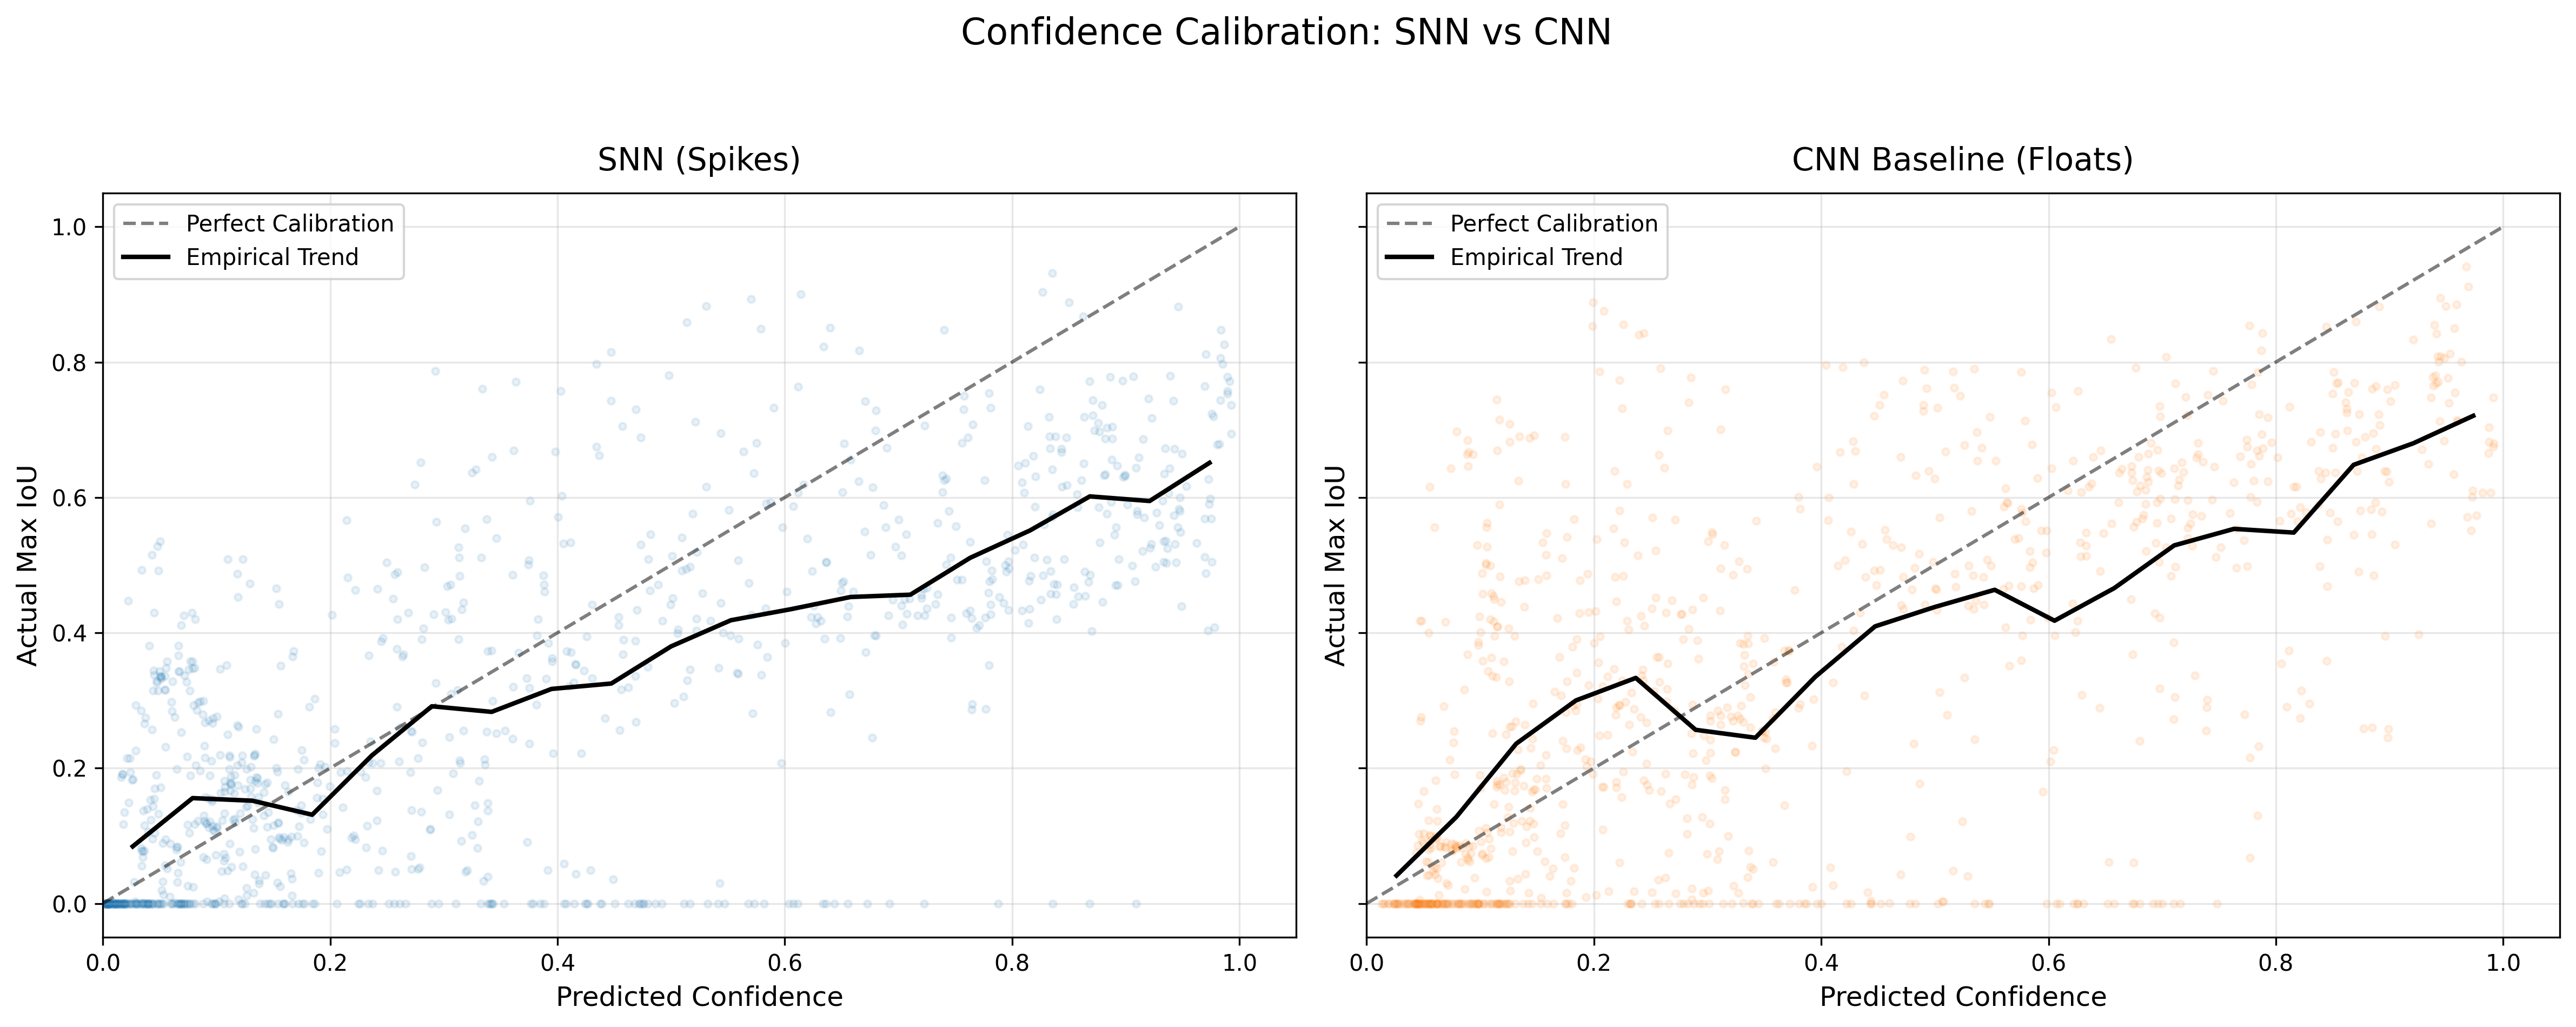
\includegraphics[width=\textwidth]{chapter_3/dnx_results/exp3_confidence_calibration.png}
    \caption[Confidence Calibration Reliability Diagrams]{Reliability diagrams for the \gls{snn} (left) and \gls{cnn} (right). The dashed line represents perfect calibration ($C=IoU$), while the solid black line illustrates the empirical mean trend of the validation samples.}
    \label{fig:confidence_calibration}
\end{figure}

\subsubsection*{Comparative Analysis: Overconfidence vs.\ Calibration}

The results demonstrate a clear divergence in predictive behavior. 
The \gls{cnn} baseline (Figure \ref{fig:confidence_calibration}, right) exhibits a pronounced \textit{overconfidence bias}: a significant density of validation samples occupy the postive-confidence region ($x > 0.5$) while maintaining an actual \gls{iou} of zero, and never predicts an $IOU=0.0$ event to have a confidence of zero. 
This indicates that the \gls{cnn} frequently hallucinates vehicle targets in background noise with near-maximum certainty, a failure mode that is critically dangerous for autonomous perception systems. 
The empirical trend line for the \gls{cnn} remains consistently below the identity line, particularly in the high-confidence domain.

In contrast, the \texttt{ULTRA} \gls{snn} (Figure \ref{fig:confidence_calibration}, left) demonstrates superior calibration, particularly at lower confidence intervals.
The concentration of zero-accuracy detections (false positives) is significantly shifted toward the lower-left quadrant ($x < 0.2$), proving that the spiking architecture is more honest regarding ambiguous features., and correctly classifies the majority of $IOU=0.0$ events with a confidence of zero.
The empirical trend line for the \gls{snn} follows a qualitatively similar trajectory to its \gls{cnn} counterpart, suggesting that the calibration behaviour is more architecture-dependent than being down to spikes versus floats.

\subsubsection*{Hypothesis Validation: The Spiking Uncertainty Sensor}

These findings validate the hypothesis formulated in Section \ref{subsec:confidence_calibration}. By utilizing discrete spike-accumulation rather than continuous floating-point intensities, the \gls{snn} acts as an implicit uncertainty sensor. Low-information features and stochastic sensor noise fail to generate a sufficient firing rate to overcome the $V_{th}=0.2$ threshold, naturally depressing the membrane potential in the regression head and resulting in lower confidence logits. 

Conversely, the \gls{cnn} utilizes exact coordinate gradients which, while providing a slight global precision advantage (as seen in Section \ref{subsec:quantization_error}), tend to overfit the confidence head to noise patterns. We can conclude that while the \gls{cnn} is more precise on average, the \gls{snn} is a fundamentally safer model, as its confidence scores are more representative of the true evidentiary strength of the input event stream.

Furthermore, both models suffer from a similar overconfidence pattern throughout the dataset due to their shared multi-box detection head, causing both to follow a similar trend trajectory as \gls{iou} increases.
This finding also exposes a direction for future work. 
Conventional detection heads, such as that employed by YOLOv8~\cite{yolov8_ultralytics}, supervise confidence as a 
scalar float logit via binary cross-entropy against hard presence labels, providing no explicit signal to align predicted confidence with localisation quality. 
An \gls{snn}-native head would instead derive confidence directly from temporal firing 
rates, naturally bounding outputs to a discrete resolution of $\frac{1}{T}$ and 
decoupling the calibration confound identified here --- divergence between the 
\gls{snn} and \gls{cnn} curves would then reflect representational differences rather 
than a shared supervisory artefact. 
A hybrid head, combining a rate-coded confidence branch with a conventional float 
regression branch, represents the most practical near-term approach.

\todo[inline]{Link to future work section.}